\section{Improve a Proactive}
	\subsection{Reason to Choose}
		Since I go to school for my appointments my biggest problem is to be on time. Therefore, this objective is one of my most important, because of this I would like to improve.
	
	\subsection{S.M.A.R.T.}
		\begin{SMART}
		    \item[Specific] A proactive for me is to be present and on time. That's one of my biggest weaknesses.
		    \item[Measurable] This can be measured by a statistical comparison of the times when I was on time and unpunctual. In addition, you can compare my arrival and absent-ness percentage together.
		    \item[Attainable] In the present time appointments, work schedules and events are an integral part and therefore time management is a very important issue.
		    \item[Relevant] This is a very relevant issue, as it could cost me my job if I am too often absent or late.
		    \item[Time-limited] The semester ends in January 2016 which is why I will have reached my goal by the end of January.
		\end{SMART}
	
	\subsection{S.T.A.R.R.}
		\begin{STARR}
		    \item[Situation] We have four Software Factory days a week were three of them goes over the whole day.
		    \item[Task] I will try to be every day in time and do not miss a day.
		    \item[Action] Most of the time I tried to be the first of my group.
		    \item[Result] As a result I create a diagram which is appended at the end of this sub section. The results are divided into "In Time", "Late" and "Not Present".
		    \item[Reflection] At the end I can say that I improved my self because at mainly each day I was present I was also the first one. In the nearer future I want to hold that and be early at work.
		\end{STARR}
		
		\begin{figure}[htbp]
			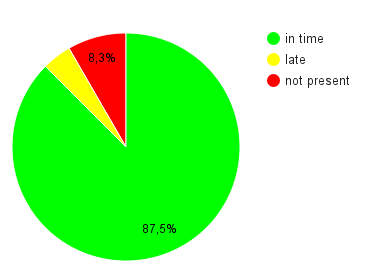
\includegraphics[width=\textwidth]{../img/inTimeDiagramm}
		\end{figure}